\documentclass[9pt, twocolumn]{extarticle}
% \documentclass[9pt, onecolumn]{extarticle}

%%% Using extarticle instead of the standard article class to allow 8pt font size
%%% Title and author fields are manually resized (e.g., \Huge, \large) for better fitting
%%% \vspace*{-\topskip} is applied in \maketitle to remove the extra top margin above the title

\usepackage{graphicx}
\graphicspath{{figs/}}
\usepackage[a4paper, margin=1.5cm, bottom=2.5cm]{geometry}
\usepackage{float}
\usepackage{subfig}
\usepackage{caption}
\usepackage{tabularx}
\usepackage{booktabs}
\usepackage[utf8]{inputenc}
\usepackage[T1]{fontenc}
\usepackage{longtable}
% \usepackage{stfloats}  % Commented out - package not available
\usepackage{amsmath}
\usepackage{titlesec}
\usepackage{setspace}
\usepackage{xcolor}
\definecolor{UofT_blue}{HTML}{0baedd}
\usepackage[colorlinks=true,
            linkcolor=UofT_blue,
            urlcolor=UofT_blue,
            citecolor=UofT_blue]{hyperref}
\usepackage[
  backend=biber,
  style=numeric,          % numbered refs
  citestyle=numeric-comp, % [1-3] compression
  sorting=none            % order of citation
  ]{biblatex}
  \addbibresource{references.bib}

\newcommand{\mystretch}{1.2}
\newcommand{\myfigmargin}{4pt}


\setlength{\textfloatsep}{\myfigmargin}    % text ↔ top/bottom floats
\setlength{\intextsep}{\myfigmargin}       % text ↔ here-placed floats ([h])
\setlength{\floatsep}{\myfigmargin}        % between floats
\setlength{\dbltextfloatsep}{\myfigmargin} % two-column floats (figure*)
\setlength{\dblfloatsep}{\myfigmargin}


\captionsetup[figure]{belowskip=0pt, skip=4pt, labelfont=bf, justification=justified, singlelinecheck=false, font={stretch=\mystretch}}
\captionsetup[subfloat]{labelfont=normalfont, justification=centering, singlelinecheck=false, farskip=4pt,captionskip=0pt, font={stretch=\mystretch}}
\captionsetup[subfloat]{belowskip=-14pt, font={stretch=\mystretch}}
\captionsetup[table]{labelfont=bf, justification=justified, singlelinecheck=false, skip=2pt, farskip=0pt, captionskip=0pt, belowskip=0pt, font={stretch=\mystretch}}
  
\renewcommand{\baselinestretch}{\mystretch} % 1.2x line spacing
  
\setlength{\columnsep}{0.5cm}
  
\makeatletter
\renewcommand\section{\@startsection{section}{1}{0pt}%
  {0.8ex plus 0.5ex minus 0.2ex}%
  {0.5ex}%
  {\normalfont\Large\bfseries}}
\makeatother


\makeatletter
\renewcommand{\maketitle}{\bgroup\setlength{\parindent}{0pt}
\vspace*{-\topskip}% remove the top margin above title
\begin{flushleft}
  \huge\textbf{\@title}

  \vspace{0.20cm}

  \normalsize\@author \hfill \normalsize\@date

  \vspace{0.25cm}\hrule\vspace{0.25cm}
\end{flushleft}
\egroup}
\makeatother


\begin{document}

% Cover Page
\begin{titlepage}
\centering
\vspace*{1.5cm}

% Title
{\fontsize{36}{42}\selectfont\bfseries\color{UofT_blue} Basin-Scale Hydrologic Characterization of La Dore (CAMELS-FR)\par}
\vspace{3.5cm}

% Author
{\fontsize{18}{18}\selectfont Ali Haghighi\par}
\vspace{2cm}

% Advisors
{\fontsize{18}{18}\selectfont Supervised by:\par}
{\fontsize{18}{24}\selectfont Afshin Ashrafzadeh\par}
\vspace{4.5cm}

% Date
{\fontsize{14}{14}\selectfont\today\par}
\vspace{2cm}

% Logos
\begin{figure}[h]
\centering
\includegraphics[height=2cm]{figs/U of T Logo.pdf}
\hspace{1cm}
\includegraphics[height=2cm]{figs/Universite de Strasbourg Logo.pdf}
\end{figure}

\vfill

\end{titlepage}

\newpage

\section*{Abstract}

This report characterizes the La Dore basin (CAMELS-FR station K287191001, 795\,km²) using CAMELS-FR attributes and time series and SRTM DEM. We describe basin physiography (morphometry, stream network, hypsometry), hydroclimate and runoff behavior (daily and monthly P, Q, PET; flow duration curve), and the long-term water balance (1990--2020). Mean annual precipitation is about 1055\,mm/yr, runoff 381\,mm/yr, and runoff ratio 0.36. Remote-sensing products (IMERG, SMAP) are reserved for future work.

% ========== 1) INTRODUCTION ==========
\section{Introduction}

Basin-scale hydrologic characterization supports water resources assessment, flood and low-flow estimation, and understanding of runoff generation. Quantifying physiography, hydroclimate, and water balance in a consistent framework provides a basis for comparison across catchments and for future use of remote-sensing products.

\textbf{Project objectives:}
\begin{itemize}
  \item Basin physiography and drainage structure (morphometry, stream network, hypsometry).
  \item Hydroclimate and runoff behavior from CAMELS-FR time series.
  \item Water balance (annual and seasonal): precipitation, runoff, PET, residual.
\end{itemize}

\textbf{Study scope.} This report uses the CAMELS-FR dataset and SRTM DEM for one focus basin (La Dore, station K287191001). IMERG and SMAP remote-sensing products are not used in the present analysis; they are reserved for future work (bias assessment, spatial representativeness, storage constraints).

% ========== 2) STUDY AREA ==========
\section{Study Area}

\subsection{Location and Boundary}
\label{sec:location}

The study basin is La Dore at Saint-Gervais-sous-Meymont (station code K287191001), catchment area 795\,km², outlet elevation 398\,m\,a.s.l.; it is one of the CAMELS-FR basins with area 500--1000\,km² (see Appendix~\ref{app:basins}). Figure~\ref{fig:basin_map} shows the catchment boundary and gauge outlet on a basemap.

\begin{figure}[htbp]
\centering
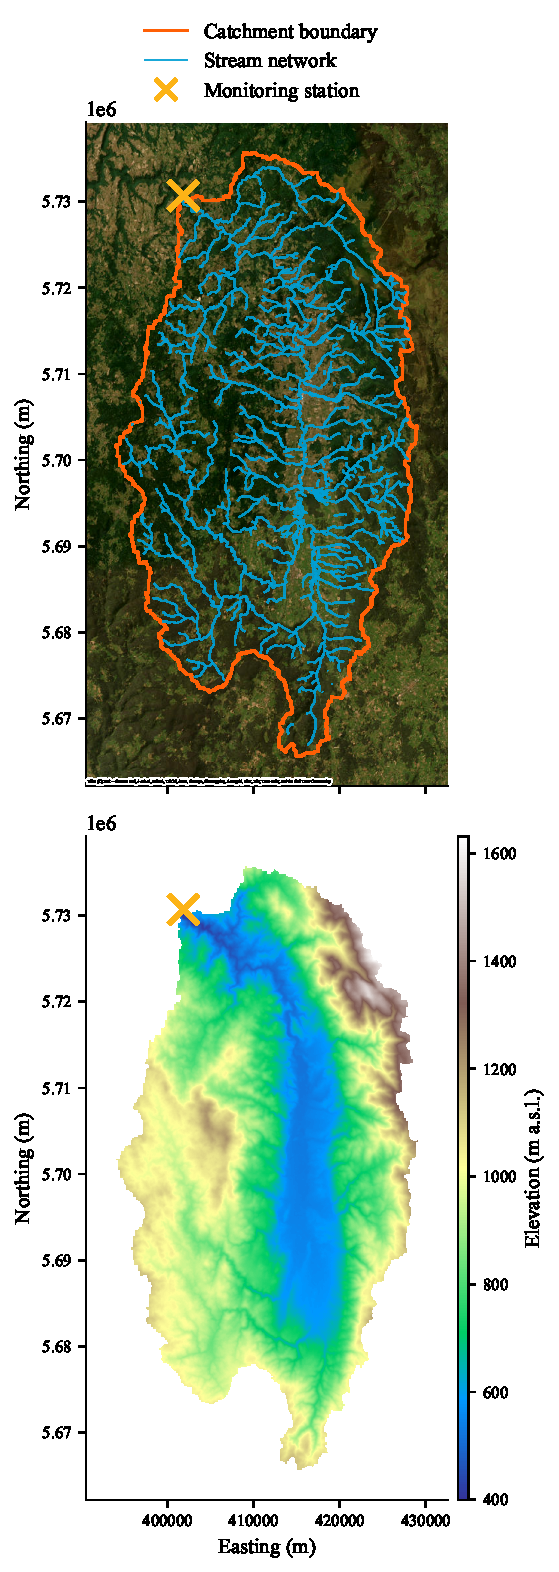
\includegraphics[width=0.95\columnwidth]{map_basin_outlet}
\caption{Catchment boundary and gauge outlet for station K287191001 (La Dore à Saint-Gervais-sous-Meymont). Area 795\,km²; outlet elevation 398\,m\,a.s.l. Map displayed in Web Mercator (EPSG:3857).}
\label{fig:basin_map}
\end{figure}

The basin lies in the Massif Central (France); coordinates at the outlet are approximately 3.61°E, 45.69°N (WGS84). The climate is temperate oceanic with continental influence; precipitation and runoff exhibit seasonal variability (winter--spring high flows, summer low flows).

\subsection{Morphometry and Shape Metrics}

Table~\ref{tab:basin_metrics} summarizes basin geometry, elevation, slope, shape, and drainage metrics. The compactness coefficient (1.88) indicates a moderately elongated shape; relief (1232\,m) and mean slope (8.5°) reflect the upland character. Drainage density (0.65\,km$^{-1}$) is typical of permeable, well-vegetated catchments.

\begin{table}[htbp]
\centering
\caption{Basin physiography and morphometric metrics for La Dore (K287191001).}
\label{tab:basin_metrics}
\begin{tabular}{ll}
\toprule
Metric & Value \\
\midrule
Area (km²) & 795.0 \\
Perimeter (km) & 188.2 \\
Basin length (km) & 31.8 \\
Main channel length (km) & 22.98 \\
Elevation min (m\,a.s.l.) & 398 \\
Elevation mean (m\,a.s.l.) & 24 \\
Elevation max (m\,a.s.l.) & 1077 \\
Relief (m) & 679 \\
Outlet elevation (m\,a.s.l.) & 398 \\
Mean slope (degrees) & 8.48 \\
Compactness coefficient & 1.88 \\
Circularity ratio & 0.28 \\
Drainage density (km$^{-1}$) & 0.6548 \\
Max Strahler order & --- \\
\bottomrule
\end{tabular}
\end{table}

\subsection{Drainage Network Characteristics}

The stream network is overlaid on the basin map (Figure~\ref{fig:basin_map}). Streams were defined by a flow-accumulation threshold of 200 cells (30\,m resolution), yielding a dendritic network consistent with the basin morphology. The main channel was traced from the outlet upstream; its length is reported in Table~\ref{tab:basin_metrics}.

\subsection{Hypsometry and Altimetry}

Figure~\ref{fig:hypsometric} shows the hypsometric curve and Figure~\ref{fig:altimetric} the cumulative area--elevation (altimetric) curve. The hypsometric integral is 0.37, indicating a basin with a relatively uniform distribution of area with elevation (neither strongly youth-like nor equilibrium). The altimetric curve shows most of the area between about 400 and 1200\,m\,a.s.l.

\begin{figure}[htbp]
\centering
\includegraphics[width=1\columnwidth]{hypsometric_curve}
\caption{Hypsometric curve: normalized elevation vs normalized cumulative area.}
\label{fig:hypsometric}
\end{figure}

\begin{figure}[htbp]
\centering
\includegraphics[width=1\columnwidth]{altimetric_curve}
\caption{Altimetric curve: cumulative area vs elevation (m\,a.s.l.).}
\label{fig:altimetric}
\end{figure}

% ========== 3) DATA ==========
\section{Data}

\subsection{CAMELS-FR}

Attributes used: station general (\texttt{sta\_area\_snap}, \texttt{sta\_altitude\_snap}), topography (elevation, slope, drainage density, compactness, form factor, etc.). Time series: daily and monthly precipitation (\texttt{tsd\_prec}, \texttt{tsm\_prec}), discharge (\texttt{tsd\_q\_mm}, \texttt{tsm\_q\_mm}), potential evapotranspiration Oudin (\texttt{tsd\_pet\_ou}, \texttt{tsm\_pet\_ou}), and temperature (\texttt{tsd\_temp}, \texttt{tsm\_temp}). Analysis period: 1990--2020 for water balance and flow duration curve; time-series snippet figure uses 2017--2020. Missing-data policy: days with missing or invalid discharge are dropped; monthly aggregates use only months with at least 90\% valid days.

\subsection{Remote Sensing}

SRTM DEM (30\,m) is used for terrain and stream network derivation. GPM IMERG and SMAP are available for future extension (precipitation bias, soil moisture); they are not used in this report.

% ========== 4) METHODS ==========
\section{Methods}

\subsection{GIS and DEM Processing}

Basin boundary and outlet are taken from CAMELS-FR geography (catchment boundaries and gauge outlet \texttt{.gpkg}). DEM preprocessing: projection to a metric CRS, optional sink filling, flow direction and flow accumulation (D8). Streams are defined by an accumulation threshold (value stated in script and below). Main channel (longest flow path) is delineated from the outlet upstream; Strahler order is assigned to the network.

\subsection{Computation of Basin Metrics}

Compactness coefficient (Gravelius): $C = P / (2\sqrt{\pi A})$, with $P$ perimeter and $A$ area. Drainage density: $D_d = \sum L / A$ (total stream length over area). Hypsometric curve: normalized elevation $(z - z_{\min})/(z_{\max} - z_{\min})$ vs normalized cumulative area; hypsometric integral is the area under this curve.

\subsection{Water Balance Framework}

Long-term: $P - Q - \mathrm{PET} \approx \Delta S$; over many years $\Delta S \to 0$. Seasonal/monthly: residual $\Delta S = P - Q - \mathrm{PET}$ (interpreted cautiously as storage change). Runoff ratio $Q/P$. Metrics: mean annual $P$, $Q$, PET (mm/yr), residual, runoff ratio, residual fraction $(P - Q - \mathrm{PET})/P$. Monthly climatology: 12-month average of $P$, $Q$, PET.

\subsection{Uncertainty and Assumptions}

Discharge is from a single gauge and is assumed representative of basin outlet runoff. Precipitation and PET are from the SAFRAN reanalysis and ISBA land-surface model (Météo-France); they are spatially aggregated to the catchment and may not capture local variability. PET (Oudin) is a potential, not actual, evapotranspiration; the residual in the water balance includes storage change and any bias in P or PET. The basin has non-negligible relief and winter precipitation; snow accumulation and melt can contribute to seasonal storage and are not explicitly separated here.

% ========== 5) RESULTS ==========
\section{Results}

\subsection{Basin Physiography}

Table~\ref{tab:basin_metrics} gives the headline metrics. Key numbers: area 795\,km², perimeter 188\,km, relief 1232\,m, mean slope 8.5°, compactness coefficient 1.88, drainage density 0.65\,km$^{-1}$. The basin is moderately elongated with substantial relief; the main channel length (about 10\,km from DEM) is shorter than the basin length (32\,km), consistent with a branched network. Over the analysis period (1990--2020), mean annual precipitation is 1055\,mm/yr, runoff 381\,mm/yr, and PET (Oudin) 592\,mm/yr; the runoff ratio $Q/P$ is 0.36 and the long-term residual fraction $(P - Q - \mathrm{PET})/P$ is about 8\%.

\subsection{Hydroclimate and Runoff Behavior}

Figure~\ref{fig:timeseries_snippet} shows discharge, rainfall, and temperature for 2017--2020 with aligned time axis. Figure~\ref{fig:climatology} shows monthly climatology; Figure~\ref{fig:fdc} the flow duration curve.

\begin{figure*}[htbp]
\centering
\includegraphics[width=1\textwidth]{timeseries_flow_precip_temp_2017_2020}
\caption{Daily time series of flow rate, rainfall, PET, and temperature (2017--2020). Shared time axis.}
\label{fig:timeseries_snippet}
\end{figure*}

\begin{figure}[htbp]
\centering
\includegraphics[width=1\columnwidth]{monthly_climatology}
\caption{Monthly climatology (1990--2020): 12-month average of precipitation, discharge, and PET.}
\label{fig:climatology}
\end{figure}

\begin{figure}[htbp]
\centering
\includegraphics[width=1\columnwidth]{flow_duration_curve}
\caption{Flow duration curve (daily Q, 1990--2020): percent of time flow is exceeded vs discharge.}
\label{fig:fdc}
\end{figure}

\subsection{Water Balance}

Figure~\ref{fig:water_balance} shows annual $P$, $Q$, PET, and residual by year. Long-term means (1990--2020): $P \approx 1055$\,mm/yr, $Q \approx 381$\,mm/yr, PET $\approx 592$\,mm/yr; runoff ratio $Q/P \approx 0.36$; residual (storage term) $\approx 82$\,mm/yr ($\sim$8\% of $P$). The positive residual on average is consistent with minor storage accumulation or uncertainty in P/PET. Seasonal residuals (from monthly climatology) reflect soil moisture and, in winter, possible snow storage.

\begin{figure*}[htbp]
\centering
\includegraphics[width=1\textwidth]{annual_water_balance}
\caption{Annual water balance: precipitation, discharge, PET, and residual (mm/yr) by year.}
\label{fig:water_balance}
\end{figure*}

% ========== 6) DISCUSSION ==========
\section{Discussion}

Runoff in La Dore is controlled by seasonal precipitation and PET (higher $Q$ in winter--spring, lower in summer), by the basin's moderate slopes and drainage density, and by storage (soil moisture, possibly snow). A runoff ratio of 0.36 is within the range typical for temperate, mid-elevation catchments. Limitations include single-gauge discharge, reanalysis-based P and PET, and the use of PET rather than actual ET. Future work with IMERG could assess precipitation bias and spatial representativeness; SMAP could constrain seasonal storage and improve water-balance closure.

% ========== 7) CONCLUSION ==========
\section{Conclusion}

\begin{itemize}
  \item Basin La Dore (K287191001): 795\,km², relief 1232\,m, compactness 1.88, drainage density 0.65\,km$^{-1}$.
  \item Hypsometric integral 0.37; stream network and main channel derived from SRTM (threshold 200 cells).
  \item Analysis period 1990--2020: mean annual P $\approx 1055$\,mm/yr, Q $\approx 381$\,mm/yr, PET $\approx 592$\,mm/yr.
  \item Runoff ratio $Q/P \approx 0.36$; residual $\approx 8$\% of $P$.
  \item Time series (2017--2020), monthly climatology, flow duration curve, and annual water balance are presented.
  \item Next steps: IMERG bias check, SMAP for storage constraint, and potential use of these data for model calibration or regionalization.
\end{itemize}

\printbibliography

\clearpage
\appendix
\onecolumn
\section{CAMELS-FR basins with catchment area 500--1000\,km²}
\label{app:basins}

The following 77 basins from the CAMELS-FR dataset have catchment area between 500 and 1000\,km² and an outlet gauge. Station code: Hydroportail \texttt{sta\_code\_h3}. Sorted by catchment area.

\textbf{Column definitions.} Outlet alt.\ is the elevation (m\,a.s.l.) of the gauge at the catchment outlet. Mean flow is mean annual runoff (mm/yr). \textbf{Agr.\ (agriculture)} is the percentage of the catchment area classified as agricultural land (CORINE Land Cover 2018, level~1), aggregated to the catchment.

\small
\begin{center}
\begin{longtable}{@{}c p{0.75cm} l >{\raggedright\arraybackslash}p{4.2cm} l r r r@{}}
\toprule
\# & Area & Code & Station (river at location) & Period & Out.\ alt (m) & Mean flow (mm/yr) & Agr.\ (\%) \\
\midrule
\endfirsthead

\multicolumn{8}{l}{\footnotesize continued from previous page} \\
\midrule
\# & Area & Code & Station (river at location) & Period & Out.\ alt (m) & Mean flow (mm/yr) & Agr.\ (\%) \\
\midrule
\endhead

\midrule
\multicolumn{8}{r}{\footnotesize continued on next page} \\
\endfoot

\bottomrule
\endlastfoot

1 & 500.1 & \texttt{A975201001} & La Nied [Française] à Condé-Northen [Pontigny] & 1968-11-01--present & 202 & 227.9 & 75.9\% \\
2 & 502.2 & \texttt{A369011001} & La Sauer à Beinheim & 1964-10-23--present & 114 & 219.4 & 23.6\% \\
3 & 506.0 & \texttt{Y503201001} & L'Argens à Châteauvert & 1971-07-01--present & 179 & 209.2 & 25.4\% \\
4 & 508.0 & \texttt{M123304010} & La Braye à Sargé-sur-Braye & 1990-05-01--present & 87 & 192.8 & 85.0\% \\
5 & 512.9 & \texttt{M313301010} & La Varenne à Saint-Fraimbault [Moulin Crinais] & 1991-06-01--present & 112 & 466.5 & 86.6\% \\
6 & 524.3 & \texttt{O234401001} & Le Girou à Cépet & 1968-09-01--present & 120 & 142.9 & 92.9\% \\
7 & 542.5 & \texttt{X043401001} & L'Ubaye à Barcelonnette [Abattoir] & 1904-01-01--present & 1134 & 577.0 & 4.5\% \\
8 & 544.8 & \texttt{O787401001} & Le Dourdou [de Conques] à Conques & 1974-11-01--present & 239 & 404.9 & 64.6\% \\
9 & 548.9 & \texttt{H032103001} & L'Ource à Autricourt & 1966-12-31--present & 196 & 353.2 & 43.4\% \\
10 & 558.8 & \texttt{F415000101} & L'Ouanne à Charny & 1968-06-01--present & 136 & 200.3 & 73.2\% \\
11 & 561.5 & \texttt{L440000101} & La Petite Creuse à Genouillac & 1967-01-01--present & 278 & 296.5 & 84.6\% \\
12 & 562.6 & \texttt{K337301001} & La Bouble à Chareil-Cintrat & 1966-07-01--present & 244 & 200.8 & 77.8\% \\
13 & 568.3 & \texttt{L510181001} & La Gartempe à Folles [Pont Gibus] & 1960-01-01--present & 282 & 433.2 & 65.1\% \\
14 & 574.9 & \texttt{K565301001} & L'Auron à Bourges - L'Ormediot & 1966-12-19--present & 128 & 184.3 & 76.3\% \\
15 & 575.7 & \texttt{J474201001} & L'Ellé à Arzano - Ty Nadan [aval pont] & 1969-01-01--present & 19 & 525.5 & 80.3\% \\
16 & 584.4 & \texttt{O509252002} & L'Aveyron à Onet-le-Château & 1967-12-31--present & 531 & 332.9 & 61.6\% \\
17 & 586.8 & \texttt{V605201001} & L'Ouvèze à Vaison-la-Romaine & 1971-02-03--present & 194 & 320.6 & 26.9\% \\
18 & 589.9 & \texttt{U221502001} & Le Dessoubre à Saint-Hippolyte & 1955-06-01--present & 383 & 725.2 & 58.6\% \\
19 & 593.4 & \texttt{K117321001} & L'Arconce à Montceaux-l'Étoile & 1969-12-01--present & 244 & 290.2 & 80.9\% \\
20 & 599.3 & \texttt{J795301020} & Le Don à Guémené-Penfao - Juzet & 1979-12-18--present & 10 & 200.6 & 89.7\% \\
21 & 607.6 & \texttt{H640203001} & La Vesle à Puisieulx & 1983-09-01--present & 85 & 136.4 & 76.0\% \\
22 & 609.4 & \texttt{U092402001} & La Vingeanne à Oisilly & 1970-12-01--present & 196 & 313.3 & 72.2\% \\
23 & 616.5 & \texttt{K633252001} & La Sauldre à Brinon-sur-Sauldre & 1987-06-01--present & 128 & 224.8 & 77.9\% \\
24 & 618.0 & \texttt{H506201001} & Le Rognon à Doulaincourt-Saucourt & 1968-08-01--present & 204 & 484.6 & 49.0\% \\
25 & 622.1 & \texttt{A330010001} & La Moder à Schweighouse-sur-Moder [aval] & 1966-05-11--present & 143 & 267.1 & 29.3\% \\
26 & 626.9 & \texttt{A420063001} & La Moselle à Saint-Nabord - Noirgueux & 1961-10-30--present & 362 & 1192.1 & 22.5\% \\
27 & 628.6 & \texttt{H612201001} & L'Aire à Varennes-en-Argonne & 1968-08-01--present & 155 & 442.3 & 73.9\% \\
28 & 646.8 & \texttt{O001004003} & La Garonne à Saint-Béat - HE & 1992-01-01--present & 507 & 1093.2 & 1.0\% \\
29 & 647.8 & \texttt{H020302002} & La Laignes aux Riceys & 1983-12-01--present & 177 & 156.1 & 61.6\% \\
30 & 662.4 & \texttt{K077322001} & Le Lignon à Poncins - Le Bourg & 1966-01-01--present & 332 & 365.2 & 47.9\% \\
31 & 668.5 & \texttt{A116003002} & L'Ill à Didenheim & 1973-10-04--present & 242 & 300.7 & 59.7\% \\
32 & 673.0 & \texttt{H512234001} & L'Ornain à Tronville-en-Barrois & 1988-12-01--present & 205 & 379.7 & 55.3\% \\
33 & 675.2 & \texttt{Y604201001} & Le Var à Entrevaux [Pont-levis] & 1920-01-01--present & 475 & 665.4 & 3.1\% \\
34 & 677.5 & \texttt{O811351001} & Le Célé à Figeac [Merlançon] & 1937-01-01--2005-01-01 & 182 & 591.4 & 63.0\% \\
35 & 684.0 & \texttt{O359402002} & Le Dourdou [de Camarès] à Vabres-l'Abbaye - Le Poujol & 1987-09-03--present & 300 & 490.2 & 42.6\% \\
36 & 686.0 & \texttt{H010002001} & La Seine à Plaines-Saint-Lange & 1967-08-01--present & 180 & 501.5 & 54.4\% \\
37 & 696.4 & \texttt{V177401001} & La Bourbre à Tignieu-Jameyzieu & 1909-01-01--present & 203 & 338.1 & 68.0\% \\
38 & 704.5 & \texttt{U233401001} & L'Allan à Fesches-le-Châtel & 1986-06-03--present & 319 & 468.4 & 34.7\% \\
39 & 722.4 & \texttt{Y028406001} & Le Tech à Argelès-sur-Mer - Pont d'Elne & 1984-08-30--present & 9 & 359.3 & 17.5\% \\
40 & 727.1 & \texttt{A615103001} & La Meurthe à Raon-l'Étape & 1973-11-01--present & 282 & 604.1 & 24.2\% \\
41 & 731.7 & \texttt{M377181010} & L'Oudon à Châtelais [Marcillé] & 1972-09-01--present & 29 & 180.0 & 93.5\% \\
42 & 734.9 & \texttt{A907105050} & La Sarre à Diedendorf & 1970-07-01--present & 220 & 320.0 & 49.5\% \\
43 & 751.1 & \texttt{H774201001} & Le Therain à Beauvais & 1967-12-31--present & 66 & 226.9 & 80.6\% \\
44 & 772.3 & \texttt{K125181001} & L'Arroux à Dracy-Saint-Loup [Surmoulin] & 1984-02-01--present & 289 & 253.9 & 72.4\% \\
45 & 791.8 & \texttt{Q219252001} & La Midouze [Le Midou] à Mont-de-Marsan & 1967-01-01--2011-03-14 & 36 & 283.3 & 70.0\% \\
46 & 792.0 & \texttt{E550572001} & L'Authie à Dompierre-sur-Authie & 1963-01-01--present & 10 & 308.3 & 88.1\% \\
47 & 795.0 & \texttt{K287191001} & La Dore à Saint-Gervais-sous-Meymont [Maison du Parc/Giroux-Dore] & 1919-01-01--present & 398 & 408.9 & 34.8\% \\
48 & 798.1 & \texttt{U464401001} & L'Azergues à Lozanne & 1964-11-17--present & 198 & 272.3 & 60.0\% \\
49 & 809.2 & \texttt{J748301001} & La Seiche à Bruz - Carcé & 1967-11-21--present & 16 & 181.8 & 89.7\% \\
50 & 810.4 & \texttt{H631302001} & La Suippe à Orainville & 1968-01-15--present & 57 & 159.2 & 82.4\% \\
51 & 816.6 & \texttt{M711241010} & La Sèvre Nantaise à Tiffauges - Ancienne Station & 1967-10-01--present & 49 & 361.0 & 91.3\% \\
52 & 832.5 & \texttt{M036151010} & L'Huisne à Nogent-le-Rotrou [Pont de bois] & 1971-11-17--present & 106 & 237.9 & 76.0\% \\
53 & 845.0 & \texttt{U122401001} & La Tille à Arceau [Arcelot] & 1966-07-01--present & 222 & 267.4 & 47.6\% \\
54 & 851.5 & \texttt{F453000101} & L'Essonne à Guigneville-sur-Essonne - La Mothe & 1974-04-01--present & 54 & 141.5 & 77.8\% \\
55 & 852.0 & \texttt{U104401001} & L'Ognon à Chassey-lès-Montbozon [Bonnal] & 1986-12-09--present & 248 & 618.7 & 37.7\% \\
56 & 853.3 & \texttt{L441171001} & La Petite Creuse à Fresselines [Puy Rageaud] & 1924-01-01--present & 222 & 297.2 & 84.7\% \\
57 & 860.7 & \texttt{K518302002} & La Tardes à Évaux-les-Bains & 1921-01-01--2008-06-01 & 385 & 317.7 & 82.8\% \\
58 & 868.0 & \texttt{H425042010} & L'Avre à Muzy & 1971-05-01--present & 80 & 127.5 & 73.9\% \\
59 & 876.2 & \texttt{Q028003001} & L'Adour à Estirac & 1968-10-01--present & 165 & 558.0 & 43.1\% \\
60 & 877.3 & \texttt{F416000201} & L'Ouanne à Gy-les-Nonains & 1968-11-22--present & 103 & 177.1 & 76.9\% \\
61 & 881.8 & \texttt{U122402001} & La Tille à Cessey-sur-Tille & 1962-12-21--present & 200 & 245.1 & 49.1\% \\
62 & 882.7 & \texttt{I522101001} & La Vire à Saint-Lô [Pont de Gourfaleur] & 1969-09-01--present & 14 & 447.8 & 91.8\% \\
63 & 884.3 & \texttt{P638251001} & L'Auvézère au Change [Aubarède] & 1964-01-01--present & 97 & 300.1 & 64.3\% \\
64 & 886.3 & \texttt{L620201002} & La Claise au Grand-Pressigny [Étableau 1] - Étableau 2 & 1976-12-31--2019-12-31 & 57 & 153.6 & 61.5\% \\
65 & 909.5 & \texttt{M005061020} & La Sarthe à Saint-Céneri-le-Gérei - Moulin-du-Désert & 1977-12-01--present & 122 & 241.1 & 82.3\% \\
66 & 917.2 & \texttt{E540031001} & La Canche à Brimeux & 1962-01-01--present & 4 & 414.6 & 86.2\% \\
67 & 929.4 & \texttt{K538302101} & L'Aumance à Hérisson - Pont de la Roche & 1969-10-01--2008-07-16 & 181 & 236.8 & 88.0\% \\
68 & 934.2 & \texttt{F467000101} & L'Orge à Morsang-sur-Orge & 1967-01-01--present & 40 & 130.6 & 44.3\% \\
69 & 937.8 & \texttt{U342401001} & La Seille à Saint-Usuge & 1968-03-01--present & 178 & 458.0 & 62.5\% \\
70 & 939.9 & \texttt{P392252001} & La Corrèze à Brive-la-Gaillarde - Pont du Buy & 1900-01-01--present & 107 & 683.1 & 43.5\% \\
71 & 943.2 & \texttt{X045401001} & L'Ubaye au Lauzet-Ubaye [Roche-Rousse] & 1959-10-01--present & 798 & 674.3 & 5.2\% \\
72 & 944.9 & \texttt{O314101001} & Le Tarn à Mostuéjouls [La Muse] & 1912-12-31--present & 398 & 921.0 & 10.4\% \\
73 & 948.1 & \texttt{A543101001} & Le Madon à Pulligny & 1964-01-01--present & 223 & 333.3 & 77.0\% \\
74 & 954.2 & \texttt{P392252002} & La Corrèze à Brive-la-Gaillarde - Le Prieur & 1918-01-01--2016-02-22 & 101 & 662.6 & 43.1\% \\
75 & 956.9 & \texttt{H616201001} & L'Aire à Chevières & 1960-01-01--present & 118 & 430.0 & 72.0\% \\
76 & 987.8 & \texttt{U303401001} & La Dheune à Palleau & 1990-10-01--present & 175 & 231.3 & 63.1\% \\
77 & 994.0 & \texttt{K259301001} & L'Alagnon à Lempdes-sur-Allagnon & 1968-01-01--present & 432 & 378.4 & 47.6\% \\
\end{longtable}
\end{center}
\normalsize

\end{document}
